\section{Operationen}
\label{sec:Kap-8.2}

In der objektorientierten Softwareentwicklung ist ein Objekt eine Einheit aus \mbox{Daten} und den Operationen, die mit diesen Daten arbeiten. Die Daten werden in den Attri\-buten gespeichert und können sich – abgesehen von Zustandsgleichheit – bei den unterschiedlichen Instanzen der Klasse auch unterscheiden. Bei den Operationen ist das anders. Die Operationen, die das Verhalten der Objekte bestimmen, sind für alle Instanzen einer Klasse identisch. Die UML bietet dementsprechend auch keine Möglichkeit, Operationen in Objekten zu modellieren, sondern nur in der zugehörigen Klasse.

Abbildung~\ref{fig:klasse_auto} zeigt die UML-Darstellung der Auto-Klasse mit den Attributen 
\linebreak %%% für Druck
\sttpUMLText{modell} und \sttpUMLText{farbe} ergänzt um die Operation \sttpUMLText{lackieren}. Für die Darstellung von Operationen wird das Rechteck der Klasse erneut horizontal unterteilt. Wie die Attri\-bute werden die Operationen linksbündig untereinander aufgeführt. 

\vspace{\baselineskip} %%% für Druck

\begin{figure}[h!]
	\centering
	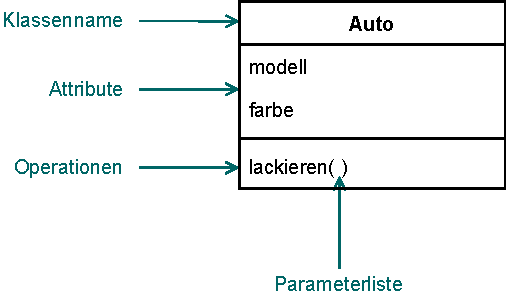
\includegraphics[scale=1.0]{Bilder/Kapitel-8/klasse_auto.pdf}
	\caption{Die Klasse \sttpUMLText{Auto} mit zwei Attributen und einer Operation}
	\label{fig:klasse_auto}
\end{figure}

Die Operationen einer Klasse spezifizieren, welche Funktionalität die Instanzen dieser Klasse anderen Objekten des Systems anbieten – technisch gesprochen: welche Funktionalität in welcher Weise aufgerufen werden kann. Man verwendet in diesem Zusammenhang auch den Begriff Dienstleistung
\marginline{Dienstleister, Dienstnutzer}
und beschreibt mit den Begriffen Dienstleister und Dienstnutzer -- die wir in Kapitel~\ref{sec:Kap-7} schon häufiger verwendet hatten --, welche Rolle ein Objekt bei Ausführung einer bestimmten Operation einnimmt. Das Objekt, das eine Operation aufruft, ist der Dienstnutzer und das Objekt, dessen Operation aufgerufen wird, ist der Dienstleister. Die entsprechende Operation (bzw. die Funktionalität, die sie abbildet) ist dementsprechend der Dienst. 

Die reine objektorientierte Modellierung abstrahiert eigentlich von dieser technischen Ebene der Operationsaufrufe und verwendet die Metapher
\marginline{Metapher\\ Nachrichten\-versand}
des Nachrichtenversands bzw. des Austauschens von Botschaften zwischen Objekten: Ein Objekt sendet eine Nachricht an ein anderes Objekt. Das die Nachricht empfangende Objekt reagiert entweder entsprechend seiner definierten Verhaltensweisen oder reagiert nicht, wenn es für die Nachricht keine definierten Verhaltensweisen besitzt. Das Konzept des Nachrichtenaustausches zwischen Objekten orientiert sich an der Realwelt: Realwelt-Objekte übermitteln verbal oder nonverbal Botschaften an andere Realwelt-Objekte (\zb die Aufforderung einer Mutter an ihr Kind, das Zimmer aufzuräumen oder der fast-verhungernde Blick eines Hundes zu seinem Besitzer) und diese reagieren auf bestimmte Art und Weise. Der Austausch von Nachrichten zwischen den Objekten in einem Softwaresystem bleibt letztendlich aber doch eine Folge von Operationsaufrufen und Operationsausführungen. Die Nachricht des Sender-Objekts besteht aus einem Operationsnamen und gegebenenfalls zusätzlichen Informationen in Form von Parametern (\su). Das Empfänger-Objekt kann auf diese Nachricht genau dann reagieren, wenn dafür eine entsprechende Operation definiert ist.\footnote{Objektorientierte Programmiersprachen verlangen in der Regel, dass nur Nachrichten gesendet werden, auf die ein Objekt auch reagieren kann. In compilierten Sprachen achtet darauf schon der Compiler. In Interpreter-Sprachen lösen Nachrichten, auf die nicht reagiert werden kann, Laufzeitfehler aus. Der Fall, dass ein Objekt eine Nachricht nicht verstehen kann, wird also im Gegensatz zur Realwelt nicht als gültige Möglichkeit angesehen.} Die Ausgestaltung der Operation bestimmt, was genau bei Eintreffen der Nachricht des Sender-Objekts passiert. 

Wir führen Operationen erst hier ein, in der Lektion zum Thema Entwurf. Das heißt aber nicht, dass man nicht auch in Domänenklassendiagrammen schon Operationen finden kann. Insbesondere in einer unspezifizierten Darstellungsform wie in Abbildung~\ref{fig:klasse_auto}, nur mit Operationsnamen und leerer Parameterliste, also ohne Parameter und ohne Angabe von Datentypen, kann man sie gut auch für Diskussionen mit den Kunden einsetzen. 

Im
\marginline{Parameter und Datentypen}
Rahmen des Entwurfs des Softwareprodukts benötigt man detailliertere Informa\-tionen zu den Operationen, da man diese sonst später nicht als Programmcode umsetzen kann. Abbildung~\ref{fig:klasse_auto_detailliert} zeigt eine erweiterte Darstellung der Auto-Klasse mit verschiedenen Möglichkeiten Parameter, Datentypen und Vorgabewerte anzugeben. Wir vermischen in dieser Abbildung verschiedene Abstraktionsebenen, um alle Aspekte an dieser einen Abbildung zeigen zu können. Eine echte Klasse sollte so nicht aussehen.

\begin{figure}[h!]
	\centering
	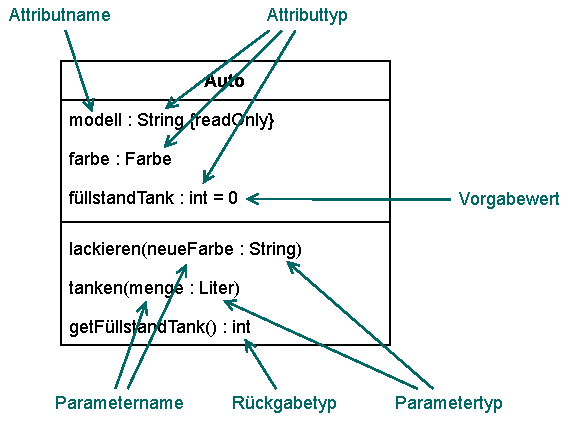
\includegraphics[scale=1.0]{Bilder/Kapitel-8/klasse_auto_detailliert.pdf}
	\caption[Die Klasse \sttpUMLText{Auto} mit detaillierteren Informationen]{Die Klasse \sttpUMLText{Auto} mit detaillierteren Informationen zu Attributen und Operationen}
	\label{fig:klasse_auto_detailliert}
\end{figure}

\pagebreak %%% für Druck

Attributnamen können um den Datentyp des Attributs (Attributtyp) ergänzt werden. Dazu wird in der UML-Darstellung hinter dem Attributnamen ein Doppelpunkt und dann der Attributtyp ergänzt. Zusätzlich kann nach dem Attributtyp auch noch ein Vorgabewert (default value) angegeben werden (wie bei \sttpUMLText{füllstandTank}). Ein Vorgabewert ist die Wertebelegung, die ein Objekt bei seiner Erzeugung erhalten soll.

Bei den Operationen können Übergabeparameter und Rückgabetypen aufgeführt werden. Die Parameter werden in gleicher Weise wie die Attribute mit Namen und Datentyp innerhalb der runden Klammern der Parameterliste der Operation angegeben. Wenn eine Operation mehrere Parameter hat, werden diese mit Komma getrennt. Je nachdem, wie implementierungsnah ein Diagramm sein soll, handelt es sich bei den Attribut- und Parametertypen schon um programmiersprachliche Datentypen (wie int und String in der Abbildung) oder noch um domänen- oder allgemeinsprachliche Angaben (wie Farbe und Liter). Gerade in Klassen\-diagrammen, die für die Kommunikation mit Nicht-Programmierern gedacht sind, finden sich häufiger Angaben wie Euro, Liter, Farbe, Grad Celsius etc. statt Integer, Float, String. Die beiden Ebenen zu mischen, wie in dieser Abbildung, ist aber eigentlich nicht sinnvoll. 

Verbund-Datentypen, die mehrere Elemente enthalten, wie Arrays oder Listen, 
\linebreak %%% für Druck
lassen sich in UML auch modellieren, allerdings in einer verallgemeinerten Form 
\linebreak %%% für Druck
über Multiplizitäten, da die UML versucht, von den verschiedenen Daten-
\linebreak %%% für Druck
strukturen konkreter Programmiersprachen zu abstrahieren. Über die Angabe 
\linebreak %%% für Druck
\sttpUMLText{[untereGrenze..obereGrenze]} lässt sich ein Datentyp entsprechend ergänzen. So bedeutet eine Angabe \sttpUMLText{int[1..5]}, dass es sich um \textbf{irgendeinen} Verbund-Datentypen handelt, in dem ein bis fünf Integer-Elemente enthalten sind. Weiter hinten im Text, in Abbildung~\ref{fig:klassen_tier_und_gehege}, wird ein solcher Datentyp verwendet. Wenn es sich um ein sehr implementierungsnahes Entwurfsdiagramm handelt und man die genaue Datenstruktur schon festlegen möchte, kann man zusätzlich mit textuellen Ergänzungen in geschweiften Klammern arbeiten. 

Ein weiterer Datentyp sind Enumerations. Eine Enumeration ist ein Datentyp mit endlichem Wertebereich, der in vielen Programmiersprachen vorkommt. Enumerations funktionieren als Aufzählungstypen, indem sie die möglichen Werte in einer Aufzählungsform angeben. Abbildung~\ref{fig:enumeration_farbe} zeigt ein Beispiel. 

\begin{figure}[h!]
	\centering
	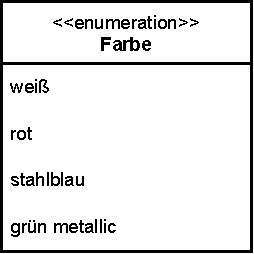
\includegraphics[scale=1.0]{Bilder/Kapitel-8/enumeration_farbe.pdf}
	\caption{Datentyp Enumeration}
	\label{fig:enumeration_farbe}
\end{figure}

\pagebreak %%% für Druck

Die UML stellt Enumerations in einer klassenähnlichen Form dar. In vielen Programmiersprachen sind Enumerations tatsächlich auch als Klassen realisiert (in \mbox{Java} auch). Das Stichwort \sttpUMLText{<<enumeration>>} in der ersten Zeile -- in UML Begriffen heißen diese \sttpUMLText{<<...>>}~-~Konstruktionen Stereotype -- signalisiert, dass es sich um eine Enumeration handelt. Die möglichen Werte werden wie die Attribute einer Klasse untereinander aufgeführt. 

\vspace{2.5mm} %%% für Druck

In der Auto-Klasse in Abbildung~\ref{fig:klasse_auto_detailliert} gab es ein Attribut \sttpUMLText{farbe : Farbe}, bei dessen Datentyp \sttpUMLText{Farbe} es sich um einen allgemeinsprachlichen Datentyp handelte. Genau auf diese Weise würde auch ein Enumerations-Datentyp angegeben, nur sollte sich dann die Information zur Enumeration (also Abbildung~\ref{fig:enumeration_farbe}) ebenfalls im Diagramm befinden bzw. anderweitig bekannt sein. Ansonsten kann dem Leser des Modells unklar bleiben, ob hier ein allgemeinsprachlicher Datentyp, eine Enumeration als Datentyp oder ein Objekt der Klasse \sttpUMLText{Farbe} -- das wird nämlich ebenso notiert -- gemeint ist.

\vspace{2.5mm} %%% für Druck

Wie detailliert (und auch wie implementierungsnah in den Bezeichnungen) ein 
\linebreak %%% für Druck
Klassendiagramm des Entwurfs ist, hängt einerseits davon ab, zu welchem Zweck es eingesetzt werden soll. Klassendiagramme, anhand derer Programmierer schon die konkrete Klassenstruktur in der Programmiersprache anlegen sollen, müssen deutlich detaillierter sein als Klassendiagramme, die als Diskussionsgrundlage über den Entwurf der Software gedacht sind. Andererseits hängt der benötigte Detailgrad \mbox{eines} Entwurf-Klassendiagramms auch davon ab, in welchem Ausmaß Artefakte aus dem Prozess des Requirements Engineering (textuelle Beschreibungen oder andere Arten von Diagrammen) vorhanden sind. Es ist zum Beispiel nicht zwingend, eine modellierte Klasse im Klassendiagramm mit allen Details auszustatten, wenn zu derselben Klasse auch eine für den Entwurf angemessene, detaillierte textuelle Beschreibung vorliegt.

\vspace{2.5mm} %%% für Druck

Wir kommen zum Thema Operationen zurück. Wie gesehen, werden die Opera\-tionen in den Klassen definiert. Zur Laufzeit des Programms werden sie dann aber auf \mbox{einem} konkreten Objekt aufgerufen. In Reaktion auf den Aufruf einer Operation zeigt dieses Objekt dann ein bestimmtes Verhalten. Dabei kann es sich auch um die Änderung seines Zustands handeln, zum Beispiel wenn in der Spezi\-fika\-tion der Operation \sttpUMLText{lackieren} steht, dass der Wert des Attributs \sttpUMLText{farbe} durch den Wert des übergebenen Parameters \sttpUMLText{neueFarbe} ersetzt werden soll. Die Reaktion auf einen Operations\-aufruf kann abhängig vom Zustand des Objekts, auf dem der Operationsaufruf durchgeführt wird, sowie abhängig von den durch das aufrufende Objekt übergebenen Parametern unterschiedlich ausfallen. So ist es zum Beispiel sinnvoll, wenn eine Auto-Instanz, deren Tank leer ist, auf einen Operationsaufruf \sttpUMLText{tanken(30 Liter)} anders reagiert als eine andere Auto-Instanz, deren Tank komplett gefüllt ist. 

\vspace{2.5mm} %%% für Druck

Man
\marginline{Selektoren, Modifikatoren}
unterscheidet Operationen, die nur lesend auf Attribute zugreifen und deren Werte nicht verändern (Selektoren) und solche, die Attributwerte verändern, also (auch) schreibend auf Attribute zugreifen (Modifikatoren). Modifikatoren ändern also den Zustand eines Objekts, Selektoren tun dies nicht. Die Operation \sttpUMLText{lackieren} ist ein Beispiel für einen Modifikator. 

\pagebreak %%% für Druck

\vspace*{\baselineskip} %%% für Druck

\begin{figure}[h!]
	\centering
	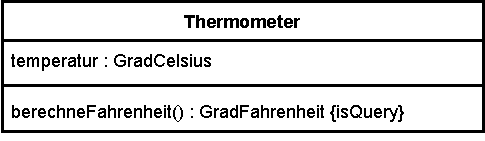
\includegraphics[scale=1.0]{Bilder/Kapitel-8/klasse_thermometer.pdf}
	\caption{Eine Selektor-Operation}
	\label{fig:klasse_thermometer}
\end{figure}

\vspace{\baselineskip} %%% für Druck

Abbildung~\ref{fig:klasse_thermometer} zeigt ein Beispiel für eine Selektor-Operation: Die Klasse \sttpUMLText{Thermometer} besitzt ein Attribut \sttpUMLText{temperatur}, das die Temperatur in der Einheit Grad Celsius enthält. Die Operation \sttpUMLText{berechneFahrenheit()} liest diesen Wert aus und errechnet daraus die Temperatur in der Einheit Grad Fahrenheit. In der UML können Selektor-Operationen durch den Zusatz \sttpUMLText{\{isQuery\}} gekennzeichnet werden. Dieser Zusatz ist aber optional. Für manche Modellierungszwecke im Laufe der Softwareentwicklung ist es nicht relevant, ob eine bestimmte Operation in der späteren konkreten Implementierung ein Selektor oder ein Modifikator werden soll.

\vspace{2mm} %%% für Druck

Die
\marginline{Getter, Setter}
„einfachsten“ Selektor- und Modifikator-Operationen sind die (eingedeutscht sogenannten) Getter und Setter. Eine get-Operation liest den Wert eines bestimmten Attributs aus und liefert diesen zurück. Eine set-Operation nimmt über einen Parameter einen Wert entgegen und ersetzt den aktuellen Wert eines bestimmten Attributs durch den Parameterwert. 

\vspace{\baselineskip} %%% für Druck
\vspace{3mm} %%% für Druck

\begin{figure}[h!]
	\centering
	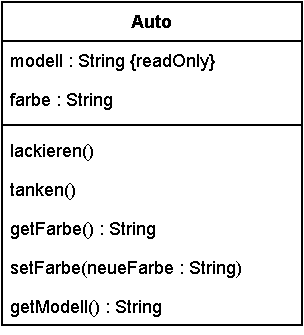
\includegraphics[scale=1.0]{Bilder/Kapitel-8/klasse_auto_getter_setter.pdf}
	\caption{get-Operationen und set-Operationen} % hier absichtlich die Kleinschreibung behalten
	\label{fig:klasse_auto_getter_setter}
\end{figure}

\vspace{\baselineskip} %%% für Druck

Abbildung~\ref{fig:klasse_auto_getter_setter} zeigt eine Klasse \sttpUMLText{Auto} mit einer get- und einer set-Operation für das Attribut \sttpUMLText{farbe}. Da das Attribut \sttpUMLText{modell} nicht veränderlich sein soll, wird für dieses Attribut keine set-Operation angelegt. Um ein Klassendiagramm nicht zu überladen, werden die Getter und Setter häufig nicht aufgeführt – oft auch in sehr implementierungs\-nahen Klassendiagrammen nicht. Die Information, zu welchen Attri\-buten einer Klasse es Getter bzw. Setter geben soll und zu welchen nicht, muss allerdings im Softwareentwicklungsteam dann anderweitig entschieden und bekannt gemacht werden.

\vspace{2mm} %%% für Druck

Get- und set-Operationen zu verwenden, anstatt auf die Attribute des Objekts \mbox{direkt} zuzugreifen, ist ein erster Schritt zur Einhaltung des Geheimnisprinzips 
\linebreak %%% für Druck
(s.~Kap.~\ref{sec:Kap-7.2.1}). Im Sinne des Geheimnisprinzips wäre es noch besser, das Wissen über vorhandene Attribute weiter zu verbergen, indem nicht mit jedem einzelnen Attribut gearbeitet, sondern auf die zu erbringende Dienstleistung fokussiert und diese über entsprechende Operationen zur Verfügung gestellt wird. Zum Beispiel würde eine Operation, die lackieren heißt (\sttpUMLText{lackieren(neueFarbe : Farbe)}), dem inhaltlichen Zweck Farbänderung aus Dienstnutzersicht erstens viel eher entsprechen als den Auftrag zu geben, ein bestimmtes Attribut zu ändern. Zweitens läge es in der Hoheit der Klasse \sttpUMLText{Auto}, diese lackieren-Operation weiter auszugestalten als nur das Attribut \sttpUMLText{farbe} zu ändern, zum Beispiel indem in einem anderen Attribut die alte Farbe des Autos dokumentiert wird oder indem der letzte Lackierungszeitpunkt gelesen wird und dementsprechend einfach oder doppelt lackiert wird etc. Den Dienstnutzer braucht nicht zu interessieren, welche Attribute wie verändert werden, solange das Auto am Ende die gewünschte neue Farbe hat. Technisch könnte man diese ganzen Dinge natürlich auch in einer setFarbe-Operation unterbringen, aber das verringert das Verständnis des Programmcodes enorm, weil niemand in einem Setter für das Attribut \sttpUMLText{farbe} anderes als eine Änderung dieses Attributs erwarten würde. 

\vspace{2mm} %%% für Druck

Wenn man jetzt noch eine Spur mehr abstrahieren möchte, folgt man den Entwurfs\-prinzipien für Schnittstellen und lässt die lackieren-Operation nicht direkt auf der Klasse \sttpUMLText{Auto}, sondern auf einer zugehörigen Schnittstelle aufrufen. Man kann aller\-dings auch Komplexität erzeugen, indem man übermäßig abstrahiert. Insofern haben Getter und Setter in jedem Fall ihre Berechtigung -- und werden auch häufig verwendet --, auch wenn sie weniger von den Implementierungsdetails einer Klasse verbergen als es mit anderen Konstruktionen möglich wäre.

\vspace{\baselineskip} %%% für Druck
\vspace{1mm} %%% für Druck

\minisec{Währenddessen im Zoo}
Wir nehmen an, im Zooprojekt ist Folgendes geschehen:

Im Prozess des Requirements Engineering hat man sich darauf verständigt, dass es zukünftig zu den Aufgaben der Tierpfleger gehören wird, die Daten der neugeborenen Tiere zu erfassen, damit diese über das Tierinformationssystem auf der Zoo-Website der Öffentlichkeit zugänglich gemacht werden können. Über ein Anwendungsfall\-diagramm wurde schon etwas differenzierter festgehalten, was ein Tierpfleger dafür mit dem Softwaresystem tun können muss (Abbildung~\ref{fig:neugeborene_tiere_erfassen}).

\begin{figure}[h!]
	\begin{addmargin*}[0cm]{-\marginparwidth}
	\begin{addmargin*}[0cm]{-\marginparsep}
		\vspace{\baselineskip} %%% für Druck
		\centering
		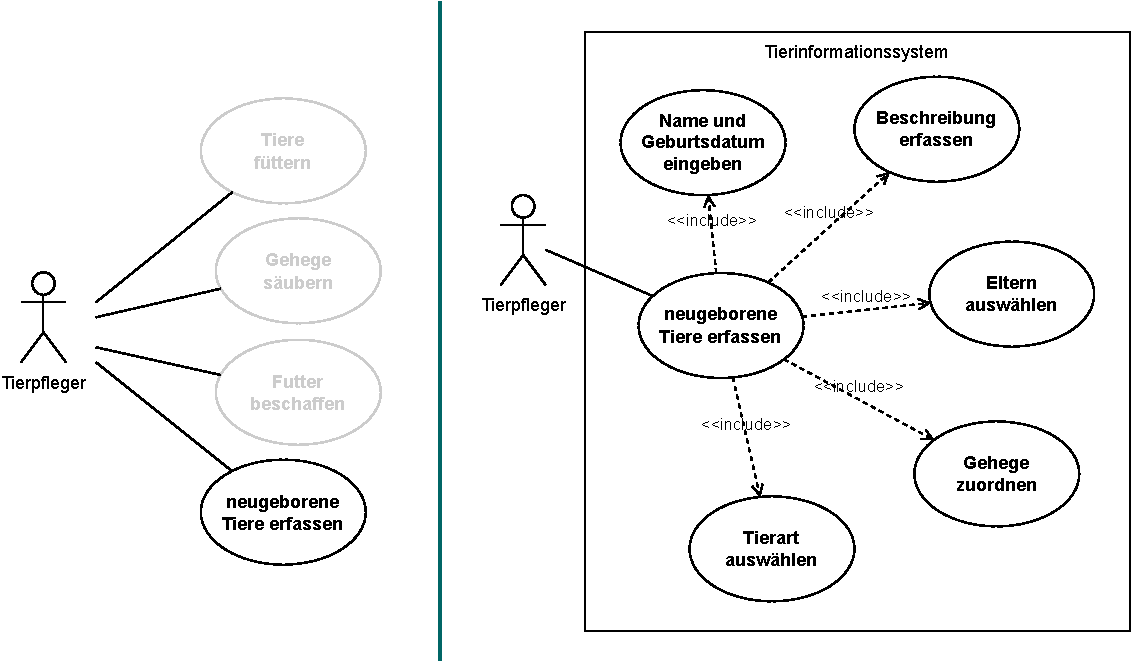
\includegraphics[scale=0.9]{Bilder/Kapitel-8/neugeborene_tiere_erfassen.pdf}
		\caption{Anwendungsfall "`neugeborene Tiere erfassen"'}
		\label{fig:neugeborene_tiere_erfassen}
	\end{addmargin*}
	\end{addmargin*}	
\end{figure}

Jetzt im Entwurfsprozess wurden die grundsätzliche Softwarearchitektur für das Tier\-informations\-system festgelegt und auch schon einige Entscheidungen zum Aussehen der Benutzungsoberfläche getroffen. Auf Grundlage aller dieser Ergebnisse ist folgende textuelle Beschreibung für den Prozess "`neugeborene Tiere erfassen"' entstanden.

\sttpUniversalkasten{Erfassung neugeborener Tiere}{
	\phantomsection
	\label{sec:Kap-8.2:Tiererfassung}
		
	Der Tierpfleger ruft die Maske \sttpUMLText{Tiererfassung} auf, um die Daten eines neugeborenen Tiers einzugeben. Er trägt in die entsprechenden Formularfelder die Stammdaten zum Tier (Name, Geburtsdatun, Größe, Gewicht) ein. Er kann auch schon eine Beschreibung der Besonderheiten des Tiers im Vergleich zu anderen Tieren derselben Art eintragen. Diese Informationen können aber auch später nachgetragen werden. Er wählt die Tierart über eine Dropdown-Liste aus. Die Eltern des Tiers wählt er über ein kontextsensitives Suchfeld mit Autovervollständigungsfunktion (freie Eingabe von Text, als Suchvorschläge werden nur Tiere derselben Tierart angegeben) aus. Er speichert die ausgefüllte Erfassungsmaske. Als letzten Schritt wechselt er auf die Übersichtsseite der Gehege und wählt dort das Gehege aus, in dem das neugeborene Tier wohnen wird. Über die Bearbeitungsfunktion auf der entsprechenden Gehege-Detailseite fügt er dem Gehege das neue Tier hinzu (anhand der aus dem vorherigen Schritt gemerkten Tier-ID oder per Auswahl aus einer Tierart-spezifischen Auswahlliste).}

\pagebreak %%% für Druck

Wir verlassen den Zoo und wechseln zurück auf die Metaebene: Aus einer solchen Beschreibung ergeben sich Objekte, deren zugehörige Klassen im Klassendiagramm berücksichtigt werden müssen. Von den Domänenobjekten sind das Tier, Gehege und Tierart. Potenzielle Kandidaten für Objekte der Benutzungsoberfläche sind Erfassungs\-maske oder Dropdown-Liste. Aber welche von denen dann schluss\-endlich durch Klassen repräsentiert werden, welche nur durch Attribute von anderen, welche reine Views sind etc., ist stark abhängig davon, mit welcher "`Technologie"' man die Benutzungsoberfläche umsetzt (selbst programmiert, über ein bestimmtes GUI-Framework, über reine HTML-Formularelemente etc.). Wir bleiben hier bei den Domänenobjekten. Für die Klasse \sttpUMLText{Tier} finden sich eine Reihe von benötigten Attri\-buten. Abbildung~\ref{fig:klasse_tier} zeigt die Klasse \sttpUMLText{Tier} mit diesen Attributen. Wir kommen auf verschiedene Aspekte dieser Tierklasse in den folgenden Abschnitten zurück. 

\vspace{\baselineskip} %%% für Druck

\phantomsection
\label{sec:Kap-8.2:Tierklasse}

\begin{figure}[h!]
	\centering
	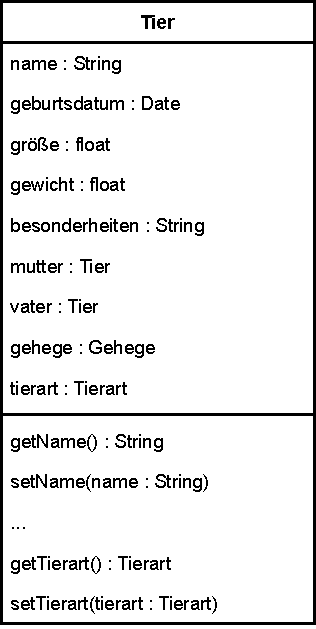
\includegraphics[scale=1.0]{Bilder/Kapitel-8/klasse_tier.pdf}
	\caption{Eine Klasse \sttpUMLText{Tier}}
	\label{fig:klasse_tier}
\end{figure}